\chapter{Metodologia}
\label{chap:metodologia}
Este capítulo apresenta a arquitetura metodológica utilizada para a condução desta pesquisa. A estrutura detalha o delineamento da pesquisa, a origem e natureza dos dados, os métodos de coleta e tratamento dos dados, os procedimentos de pré-processamento e agregação, a engenharia de variáveis desenvolvida para aprofundar a análise e, por fim, as técnicas de estatística inferencial empregadas para testar hipóteses e construir um modelo preditivo. Cada etapa é descrita com o objetivo de garantir a transparência e a replicabilidade do estudo. Além de especificar softwares e bibliotecas utilizadas.

\begin{figure}[h!]
    \centering
    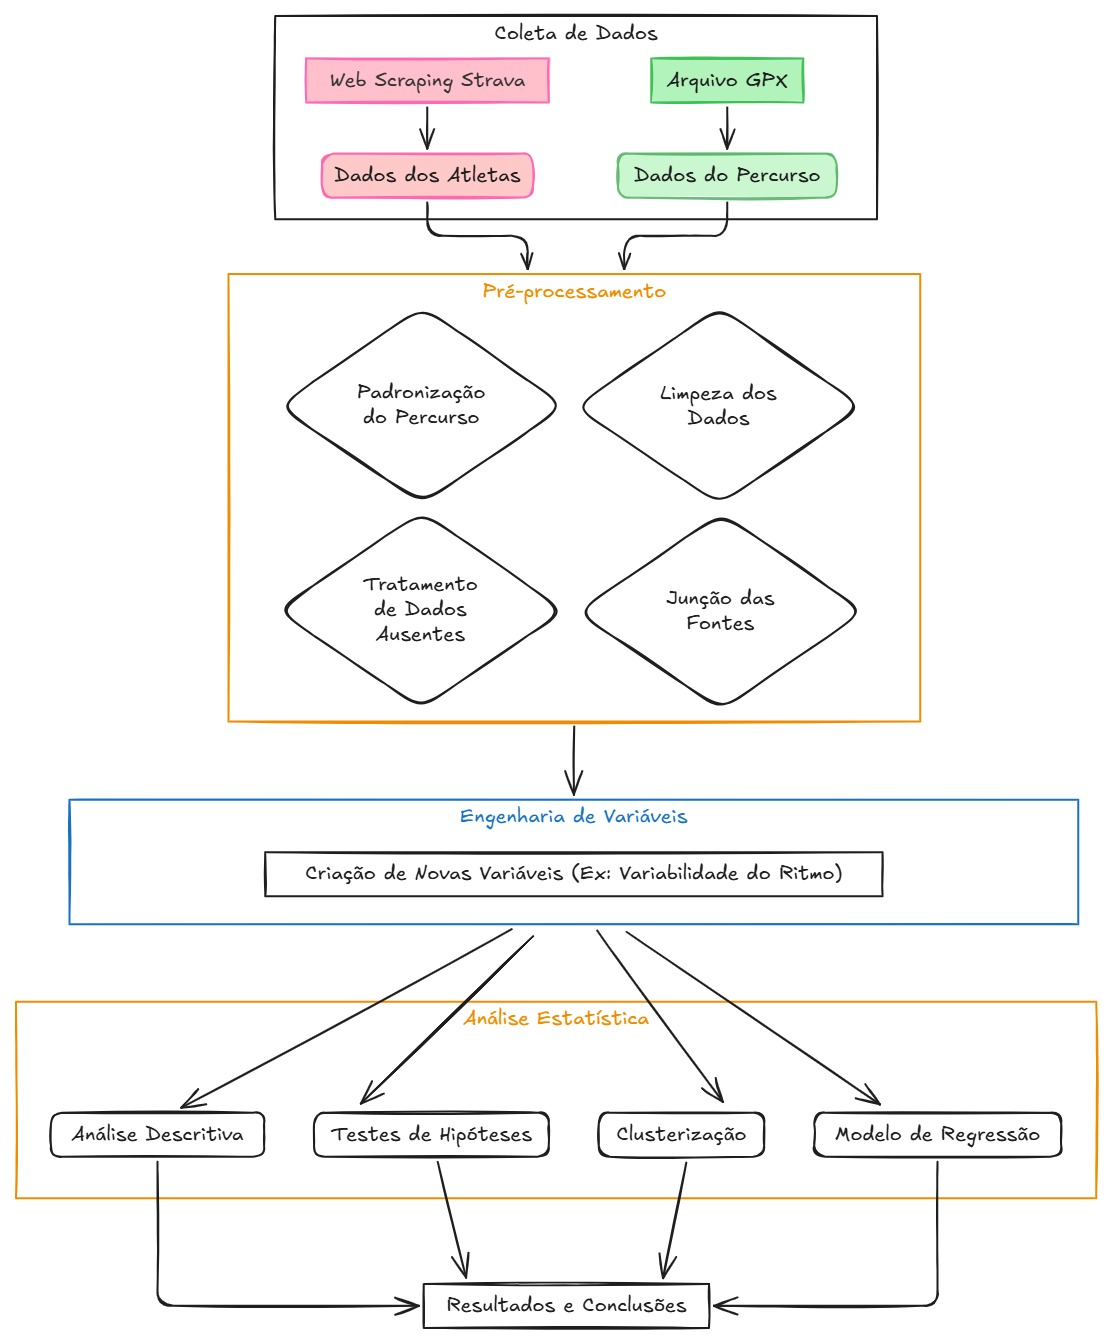
\includegraphics[width=0.75\textwidth]{Imagens/fluxo_trabalho.png}
    \caption{Fluxograma do processo de coleta e análise de dados. Fonte: Elaborado pelo autor (2025).}
    \label{fig:fluxograma}
\end{figure}

\section{Delineamento da Pesquisa}

Foi realizado um estudo quantitativo, de caráter descritivo e explicativo. Descritivo por meio da Análise Exploratória de Dados (AED), que visa caracterizar o perfil dos atletas da amostra. Explicativo ao utilizar técnicas de estatística inferencial, como a regressão linear múltipla, para modelar e explicar a relação entre um conjunto de variáveis e o desempenho final dos corredores.

\section{Fonte e Natureza dos Dados}
\label{sec:fonte_dados}

Os dados utilizados neste estudo foram extraídos da plataforma de rastreamento de atividades físicas Strava, referentes às edições de 2022 e 2023 da prova de \emph{trekking} de montanha \textit{La Misión Brasil}, na modalidade de 35 quilômetros. A extração foi realizada por meio de técnicas de \emph{web scraping}, conforme detalhado na Seção \ref{subsec:scraping}.

A natureza do conjunto de dados original era granular, com cada linha representando o desempenho de um único atleta em um quilômetro específico da prova. Essa estrutura, embora detalhada, não era adequada para uma análise centrada no desempenho geral do atleta, necessitando de uma etapa de agregação.

\section{Coleta e Pré-processamento dos Dados}

A obtenção dos dados foi dividida em quatro fases principais: padronização das informações do percurso, extração automatizada de dados da web, limpeza e estruturação final do conjunto de dados.

\subsection{Padronização dos Dados do Percurso via GPX}
\label{subsec:gpx}

A fim de garantir a consistência e a padronização das variáveis geográficas do percurso para todos os atletas, evitando discrepâncias inerentes a diferentes dispositivos de GPS, o ponto de partida foi a análise de um arquivo GPX (GPS Exchange Format) oficial da prova. Este arquivo foi processado para extrair informações de elevação a cada quilômetro, criando um gabarito do percurso com 36 segmentos. Essa abordagem permitiu que variáveis como ganho de elevação positivo e negativo de um determinado quilômetro fossem padronizadas e atribuídas de forma idêntica a todos os corredores da amostra.

\subsection{Extração de Dados via \textit{Web Scraping}}
\label{subsec:scraping}
Para a extração dos dados de desempenho e demográficos dos atletas, foi desenvolvida uma solução de \emph{web scraping} utilizando a linguagem de programação Python e a biblioteca \texttt{Selenium}, que permite a automação de navegadores web. O processo exigiu a autenticação em uma conta de usuário com assinatura paga na plataforma Strava para acessar os dados detalhados. O fluxo de extração foi estruturado da seguinte forma:

\begin{figure}[h!]
    \centering
    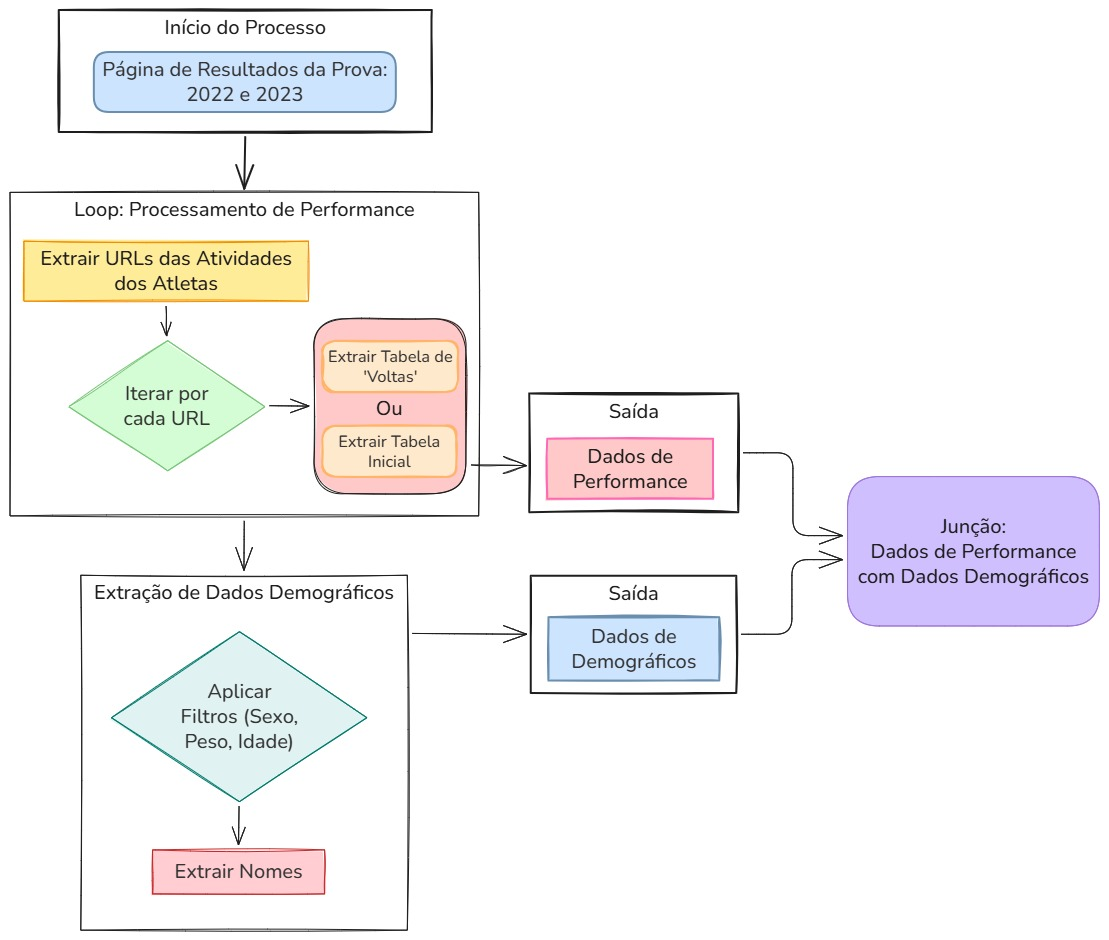
\includegraphics[width=0.7\textwidth]{Imagens/fluxo_webscraping.png}
    \caption{Fluxograma do processo de Web Scraping. Fonte: Elaborado pelo autor (2025).}
    \label{fig:fluxograma}
\end{figure}

\begin{enumerate}
    \item \textbf{Coleta de Links:} O ponto de partida foram as páginas de resultados (tabelas de classificação) das edições de 2022 e 2023 da prova. O script navegou por estas páginas e coletou as URLs individuais de cada atividade de atleta registrada.
    
    \item \textbf{Extração de Dados de Performance:} Em um processo iterativo, o script acessava a URL de cada atleta. A prioridade era extrair a tabela de ``Voltas'' (\texttt{laps}), identificada pelo seletor CSS \texttt{'li[data-tracking-element="laps"] a'}, que continha os dados detalhados de tempo a cada quilômetro. Caso esta tabela não estivesse disponível, o script adotava uma abordagem de \emph{fallback}, extraindo os dados da tabela de segmentos principal.
    
    \item \textbf{Extração de Dados Demográficos:} Para obter as variáveis de sexo, faixa etária e faixa de peso, foi empregada uma técnica de filtragem na página principal de resultados. O script aplicava sequencialmente cada filtro (ex: sexo masculino), extraía a lista de nomes dos atletas correspondentes e armazenava essa informação. Posteriormente, esses dados foram unificados com os dados de performance através do nome dos atletas.
    
    \item \textbf{Gestão de Desafios Técnicos:} Durante a execução, foi observado que a plataforma poderia apresentar lentidão no carregamento de elementos. Para contornar essa questão, pausas estratégicas de 5 segundos (\texttt{time.sleep(5)}) foram inseridas no código para garantir que as páginas estivessem completamente carregadas antes da extração, aumentando a robustez do processo.
\end{enumerate}
Importante ressaltar que a coleta foi restrita a dados de perfis e atividades publicamente compartilhados pelos usuários.

\subsection{Limpeza e Estruturação dos Dados}
\label{subsec:limpeza}

Após a extração, foi realizado um rigoroso processo de limpeza e estruturação:
\begin{enumerate}
    \item \textbf{Unificação e Junção:} Os dados de performance dos atletas foram unidos (\emph{join}) aos dados padronizados do percurso (obtidos via GPX) pela coluna indicativa do quilômetro.
    
    \item \textbf{Tratamento de Duplicatas:} Identificou-se que 7 atletas participaram das duas edições da prova. Para garantir a independência das observações, foi mantida apenas a primeira participação de cada um, resultando em 166 atletas únicos nesta fase.
    
    \item \textbf{Padronização de Variáveis:} As colunas de `Tempo` e `Ritmo`, que se apresentavam em formatos distintos, foram unificadas e convertidas para uma unidade padrão de segundos.
    
    \item \textbf{Tratamento de Valores Ausentes:} A estratégia de tratamento de dados faltantes foi definida conforme a variável:
    \begin{itemize}
        \item \textbf{Frequência Cardíaca:} A coluna foi removida do conjunto de dados devido ao alto percentual de valores ausentes.
        \item \textbf{Faixa de Peso:} Com aproximadamente 12,44\% de dados faltantes, optou-se por imputar os valores nulos com a categoria ``Não Informado'', por se tratar de uma variável relevante para a análise.
        \item \textbf{Sexo e Faixa Etária:} Devido ao baixo percentual de ausência (inferior a 10\%), os atletas (linhas) sem essas informações foram removidos do estudo (exclusão \emph{listwise}).
    \end{itemize}
\end{enumerate}
Ao final deste processo, consolidou-se um conjunto de dados final, limpo e estruturado no formato \emph{long}, contendo 109 atletas e 36 observações (quilômetros) para cada um.

\subsection{Agregação dos Dados}
\label{sec:preprocessamento}

Para transformar os dados granulares em um formato analítico focado no atleta, foi realizado um processo de agregação. Utilizando uma operação de agrupamento (\texttt{groupby}) por identificador de atleta, o conjunto de dados foi consolidado, passando de uma estrutura por quilômetro para uma estrutura em que cada linha representava um único atleta. Nesta etapa, foram criadas as variáveis agregadas fundamentais para a análise:
\begin{itemize}
    \item \textbf{\texttt{Tempo\_Final\_seg}:} Variável dependente principal do estudo, calculada como a soma total do tempo de cada quilômetro percorrido pelo atleta.
    \item \textbf{\texttt{Ritmo\_Medio\_seg}:} A média do tempo, em segundos, por quilômetro.
    \item \textbf{\texttt{Variabilidade\_Ritmo\_std}:} O desvio padrão do tempo por quilômetro, servindo como a principal métrica de consistência do ritmo do atleta ao longo da prova.
\end{itemize}

\section{Engenharia de Variáveis}
\label{sec:engenharia_variaveis_final}

Após feita a coleta de dados, assim como seu tratamento, foi realizado a etapa crucial da análise que consistiu na elaboração de novas métricas para capturar nuances da estratégia de prova e da performance dos atletas em diferentes terrenos. 

\subsection{Variáveis de Estratégia de Prova (\textit{Splits})}

Para analisar a distribuição de esforço, a prova foi dividida em duas metades: "Primeira Metade" (quilômetros 1-18) e "Segunda Metade" (quilômetros 19-36). A partir dessa segmentação, foram criadas as variáveis \texttt{Ritmo\_Medio\_Primeira\_Metade} e \texttt{Ritmo\_Medio\_Segunda\_Metade}.

Para uma comparação mais robusta da variação de ritmo, foi criada a variável \texttt{diff\_relativa\_segunda\_primeira\_parte}. A justificativa para o uso de uma métrica relativa, em vez de uma diferença absoluta, reside no fato de que uma mesma variação de tempo (e.g., 30 segundos) possui significados distintos para um atleta de elite e um amador. A normalização pelo ritmo médio do próprio atleta gera uma medida de eficiência de \emph{pacing} mais justa e comparável entre corredores de diferentes níveis de habilidade.

\subsection{Variáveis Baseadas em Terreno (Altimetria)}

Para isolar o desempenho em diferentes inclinações, cada quilômetro do percurso foi classificado como "SUBIDA", "DESCIDA", "PLANO" ou "MISTO". Essa classificação foi realizada por uma função customizada (\texttt{Sob\_Desc}) baseada em regras sobre o desnível positivo e negativo de cada trecho. A partir dessa categorização, foram calculadas as variáveis de ritmo médio para cada tipo de terreno, como \texttt{Ritmo\_Medio\_SUBIDA} e \texttt{Ritmo\_Medio\_DESCIDA}.

\subsection{Índices de Performance Relativa}

Visando quantificar a especialização técnica dos atletas, foram desenvolvidos índices normalizados que comparam o desempenho em terrenos específicos com o desempenho geral do próprio indivíduo.
\begin{itemize}
    \item \textbf{\texttt{indice\_subida}:} Mede o quão mais lento um atleta é na subida em comparação com sua própria média geral.
    \item \textbf{\texttt{indice\_descida}:} Mede o quão mais rápido um atleta é na descida em comparação com sua média geral.
    \item \textbf{\texttt{indice\_descida\_vs\_subida}:} Compara diretamente a performance nos dois terrenos-chave, servindo como uma métrica da capacidade de aceleração relativa do atleta em descidas versus subidas.
\end{itemize}

\section{Análise Estatística}
\label{sec:analise_estatistica}

A análise dos dados foi conduzida por meio de um conjunto de técnicas estatísticas, onde a escolha de cada teste foi rigorosamente justificada pelos pressupostos dos dados.

\subsection{Análise Descritiva}
Inicialmente, foi realizada uma análise descritiva com o uso de medidas de tendência central (média, mediana) e dispersão (desvio padrão) para as variáveis quantitativas, e distribuições de frequência para as variáveis categóricas. Visualizações gráficas como histogramas, diagramas de dispersão e \emph{boxplots} foram utilizadas para compreensão visual dos dados e distribuição das variáveis.

\subsection{Testes de Hipóteses}
\begin{itemize}
    \item \textbf{Comparação entre Sexos:} Para comparar a variável \texttt{Tempo\_Final\_min}, o pressuposto de normalidade foi verificado com o teste de Shapiro-Wilk. A violação do pressuposto (p < 0.05 para ambos os grupos) levou à escolha do teste não-paramétrico de Mann-Whitney U, apropriado para a comparação de duas amostras independentes sem distribuição normal.
    \item \textbf{Comparação entre Faixas Etárias:} Seguindo a mesma lógica, a não-normalidade dos grupos, verificada pelo teste de Shapiro-Wilk, justificou o uso do teste de Kruskal-Wallis. Para investigar as diferenças específicas entre os pares de grupos, foi aplicado o teste \emph{post-hoc} de Dunn com correção de Bonferroni para o controle da taxa de erro do tipo I.
    \item \textbf{Comparação entre Faixas de Peso:} Visando verificar se existe diferença entre as faixas de peso, com a não-normalidade dos grupos, verificada pelo teste de Shapiro-Wilk, justificou o uso do teste de Kruskal-Wallis.
\end{itemize}

\subsection{Análise de Associação}
Para investigar a relação entre performance, \texttt{Tempo\_Final\_min}, e consistência do ritmo, \texttt{Variabilidade\_Ritmo\_min\_std}, a não-normalidade de ambas as variáveis, indicada pelo teste de Shapiro-Wilk, determinou o uso da Correlação de Spearman ($\rho$). Este teste foi escolhido por sua adequação para avaliar avalia a força e a direção das relações monotônicas, independentemente da distribuição dos dados, em contraste com a correlação de Pearson, que pressupõe uma relação linear e normalidade.

\subsection{Análise de Agrupamento}

Com o objetivo de identificar perfis distintos de corredores ("personas") com base em suas características de prova, foi aplicada a técnica de clusterização não-supervisionada K-Means. O propósito desta análise foi segmentar a amostra em grupos intrinsecamente homogêneos e extrinsecamente heterogêneos, revelando diferentes estratégias e especialidades de desempenho dos atletas.

\subsubsection{Pré-processamento das Variáveis para Clusterização}

O algoritmo K-Means agrupa os dados minimizando a variância intra-cluster, um processo que se baseia fundamentalmente no cálculo de distâncias (tipicamente a distância Euclidiana) entre as observações e os centróides dos clusters. Quando as variáveis de entrada (features) possuem escalas e magnitudes muito diferentes — como, por exemplo, uma variável de tempo em segundos (na casa dos milhares) e um índice de performance (na casa de 0.1 a 0.3) — o cálculo da distância pode ser enviesado. A variável com a maior magnitude iria dominar o cálculo, minimizando ou até anulando a contribuição das outras variáveis para a definição dos grupos.\citep{muller2016}.

Para suavizar este efeito e garantir que todas as variáveis tivessem a mesma importância relativa no processo de agrupamento, foi realizado um pré-processamento de padronização dos dados por meio da técnica \textit{StandardScaler}. Este método transforma cada variável para que ela passe a ter uma média igual a zero e um desvio padrão igual a um. A escolha por essa técnica se justifica pois muitos algoritmos de aprendizado de máquina assumem que as características estão centradas em zero e possuem variância na mesma ordem, evitando que uma variável domine a função objetivo do algoritmo \citep{scikitlearn_preprocessing}. A fórmula para a padronização de cada observação (x) em uma variável é dada por:

\begin{equation}
    z = \frac{x - \mu}{\sigma}
    \label{eq:standardscaler}
\end{equation}

Onde:
\begin{itemize}
    \item $z$ é o valor padronizado (ou z-score);
    \item $x$ é o valor original da observação;
    \item $\mu$ é a média de todos os valores da variável (feature);
    \item $\sigma$ é o desvio padrão de todos os valores da variável.
\end{itemize}

Este passo metodológico foi crucial para assegurar que a formação dos clusters fosse resultado dos padrões nos dados, e não de uma distorção causada pelas diferentes escalas das métricas de desempenho.

\subsubsection{Seleção do Número de Clusters (k)}

A determinação do número ideal de agrupamentos ($k$) é um parâmetro fundamental para o algoritmo K-Means. Para esta finalidade, foi empregado o Método do Cotovelo (\textit{Elbow Method})\citep{thorndike1953}. Este método consiste em executar o algoritmo de clusterização para um intervalo de valores de $k$ (e.g., de 1 a 10) e calcular a soma dos quadrados das distâncias intra-cluster (inércia) para cada valor. O número ótimo de clusters é visualmente identificado no ponto do gráfico onde a adição de um novo cluster não resulta em uma diminuição significativa da inércia, formando um "cotovelo" na curva.


\subsection{Modelagem Preditiva}
Para atingir o objetivo principal do trabalho, foi ajustado um modelo de regressão linear múltipla para prever o tempo final dos atletas (variável dependente) a partir de um conjunto de variáveis preditoras (independentes). Para desenvolver um modelo capaz de prever a variável \texttt{Tempo\_Final\_seg}, foi empregada a técnica de Regressão Linear Múltipla, ajustada por Mínimos Quadrados Ordinários (OLS).
\begin{itemize}
    \item \textbf{Refinamento do Modelo:} Partindo de um modelo inicial com múltiplas variáveis, foi aplicado um processo de seleção de variáveis \emph{backward elimination} (eliminação retrógrada), removendo iterativamente os preditores não significativos (com p-valor > 0.05). Adicionalmente, a multicolinearidade entre as variáveis remanescentes foi verificada por meio do Fator de Inflação de Variância (VIF), assegurando a obtenção de um modelo final parcimonioso, robusto e de fácil interpretação.
    \item \textbf{Avaliação do Modelo:} A avaliação do modelo final foi realizada por meio da significância estatística dos coeficientes, da análise do coeficiente de determinação ajustado ($R^2$ ajustado) e da análise gráfica dos resíduos. A análise dos resíduos incluiu a verificação de homocedasticidade, normalidade e independência, garantindo que os pressupostos da regressão linear fossem atendidos.
\end{itemize}

\section{Softwares Utilizados}

Todas as etapas de coleta, tratamento e análise estatística dos dados foram conduzidas na linguagem de programação Python (versão 3.x), com o auxílio de bibliotecas consagradas para manipulação e análise de dados, como Pandas, NumPy, Matplotlib, Seaborn, e para modelagem estatística, como Scikit-learn e Statsmodels.

% --- FIM DO CAPÍTULO DE METODOLOGIA ---